% section 2: Components

\section{Components}  \label{sec:components}

The DC3a Alert Production is accomplished through a set of
\textit{pipelines} that work together which collectively we refer to
as a \textit{production}.  A \textit{production run} is a particular
instantiation and execution of those pipelines that produces a
collection of data products, which in the case of alert production are
the calibrated images and a catalog of detected objects.  A
\textit{pipeline} itself is a series of processing steps (called
\textit{stages}) which are cyclically applied to a sequence of data
chunks.  Since alert production is meant to run in real time on data
coming from the telescope, the chuncks of data to be processed are the
so-called \textit{visits}, in which each visit is comprised of two
15-second exposures of the same field in the sky.  Each visit,
generally, is different field in the sky.    
Figure \ref{fig:dc3apipes} diagrams major components of the processing flow in DC3a;
figure \ref{fig:lsstpipes} shows for comparison the baseline design for processing 
flow in the fully implemented LSST.

Building on the design from DC2, the Alert Production is comprised of
three pipelines: 

\begin{itemize}

\item The \textit{image processing and source detection} (IPSD)
  pipeline takes as input the raw exposure images along with the
  related calibration data and produces a catalog of the light sources
  found within those images. DC3a added image signature removal to
  this pipeline, along with the paradigm of processing both exposures
  the make up the visit and use them to detect cosmic ray defects.

\item The \textit{Night Moving Object Processing System} pipeline
  (NightMOPS) takes time and coordinate information from the exposure
  and creates a catalog of known solar system objects expected to be
  within the exposure FOV. It operates in parallel with the IPSD
  pipeline.

\item The \textit{association pipeline} (AP) then correlates the
  sources found by the IPSD with known objects --- either fixed
  objects or objects expected by NightMOPS to be within the FOV --- to
  determine whether new sources have been detected.

\begin{figure}[t]
\begin{center}
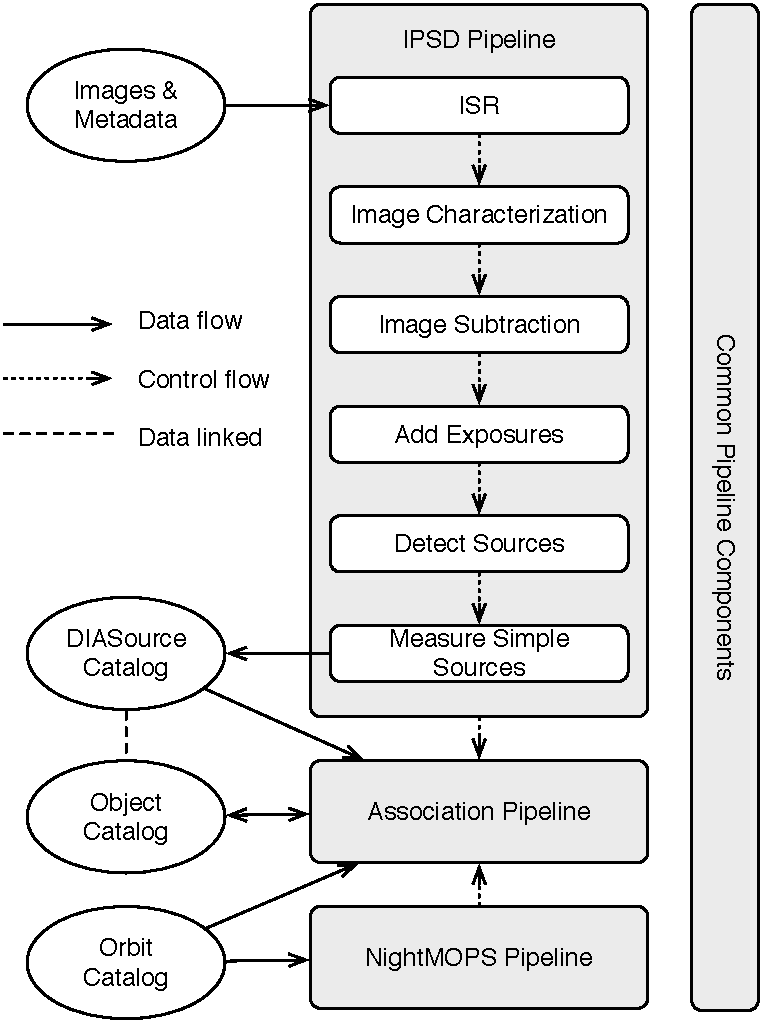
\includegraphics[width=3in]{images/DC3aNightly.pdf}
\caption{Processing flow in DC3a. Three pipelines (IPSD, Association, and
NightMOPS) are supported by a common infrastructure.  
\label{fig:dc3apipes}}
\end{center}
\end{figure}

\begin{figure}[t]
\begin{center}
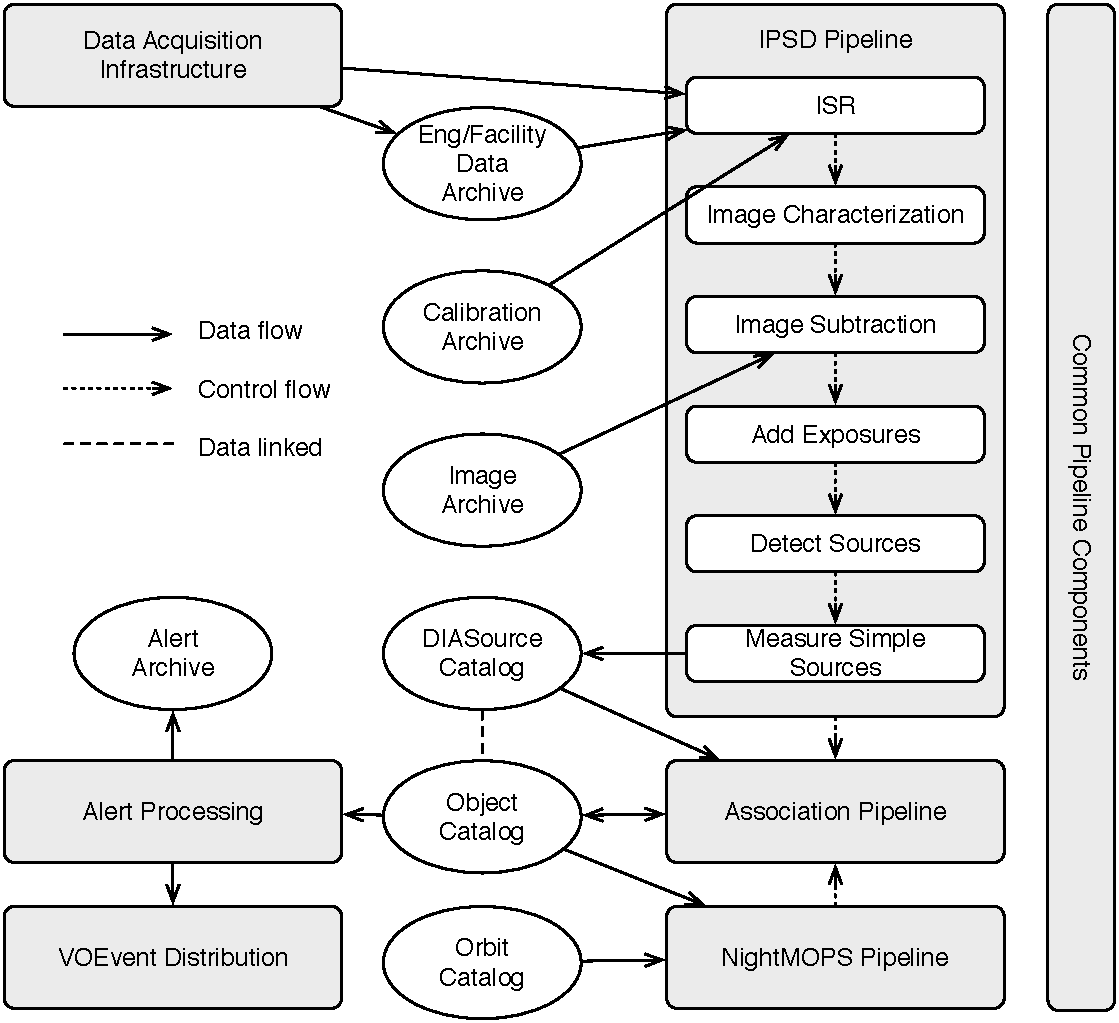
\includegraphics[width=4.5in]{images/LSSTpipes.pdf}
\caption{Baseline design for nightly image processing flow for LSST; DC3a represents
a subset of this design.  
\label{fig:lsstpipes}}
\end{center}
\end{figure}


\end{itemize}

A pipeline can process data in highly parallelized manner; in general,
a pipeline will use a consistent model of data parallelism, in which a
parallel process (a \textit{slice}) will operate on the same logical
portion of the input dataset throughout all the pipeline stages.  For
example, each slice in the IPSD pipeline processes a different
amplifier segment of a CCD that comprises the focal plane.  The
NightMOPS pipeline distributes the known objects in its catalogue
across its slices.  

The three pipelines run simultaneously on different machines but are
loosely coupled via event-based communication.  In particular, the
IPSD and NightMOPS pipelines will process the next visit when they
receive an external event message indicating that a new visit is
available for processing.  These pipeline both emit an event message
when they have finished processing a visit.  These events are picked
up by the AP pipeline as a signal that there are new detections in the
database to be associated with known objects.  The routing of these
event messages between pipelines is facilited by an \textit{event
broker} (which runs as a separate process).  

Events are also used for collecting logging messages from all of the
processes that make up the pipelines.  A special \textit{event
monitor} program collects these messages and loads them into the
database.  

The whole production is configured via a set of human-readable
\textit{policy files} which provide values for parameters that
configure the behavior of the various pipeline components.  In
particular, a production-level policies defines the pipelines that
make up the production along with the properties of the platforms that
they will run on.  Pipeline-level policies define the stages that make
up each pipeline along with details for setting up the pipeline for
execution.  Each stage also has a policy that sets various parameters
used by algorithms that will be applied to the data.  

Data Products come in two forms: FITS images and records into a
database.  A shared MySQL database is used for the latter.  In
particular, insert into and retrieval from the database is the main
mechanism for passing object and source information betweeen
pipelines.  

\subsection{Overview of Processing Flow}

In this section, we take a closer look how the different software
components work together to process the sequence of visits that come
from the telescope.  

\subsubsection{Middleware for Launching and Managing Pipelines} 
\label{sec:orcaintro}

The \textit{orchestration layer} is responsible for configuring,
preparing, launching, and monitoring the pipelines that make up a
production.  In general, each pipeline can be deployed on a different
platform, so the orchestration layer must be able to adapt to
different platforms and operate remotely.  The layer is implemented
via the \texttt{ctrl\_orca} software package (short for
``Control-Orchestration''; see section \ref{sec:PipelineOrchestration})
and initiated via its \texttt{orca.py} launch script.  This basic
inputs to this script includes a production-level policy file
(\texttt{dc3pipe.paf}) which contains pointers to all the other policy
files needed to configure the pipelines.  Another important input is
the \textit{run identifier} (or ``run-ID'', for short) which is a
short name that identifies a particular instantiation of the pipelines
and the overall collection of data products they will produce.  When
executed, the script will:  

\begin{itemize}
\item Create working directories on the target platforms for input and
  output data, policy files, and log files,
\item Initialize the database tables to be used by the pipelines, 
\item Deploy all needed policy files and launch scripts onto the
  target platforms,
\item Set the necessary software environment, and 
\item Remotely execute each platform launch script.
\end{itemize}

For DC3a, the \texttt{orca.py} script was executed through another
script called \texttt{launchDC3a.py} from the \texttt{ctrl\_dc3pipe}
package.  This script handles setup that is specific to DC3a.  In
particular, after executing the \texttt{orca.py} script, it runs
another script that creates and emits the ``data-is-available'' events
that trigger the IPSD and NightMOPS pipelines to start processing.
(During actual production operation of the observatory, these events
would be generated by the observatory control software.)  These events
are emitted at a specified cadence to simulate retrieval of data from
the telescope.  

\begin{figure}[t]
\begin{center}
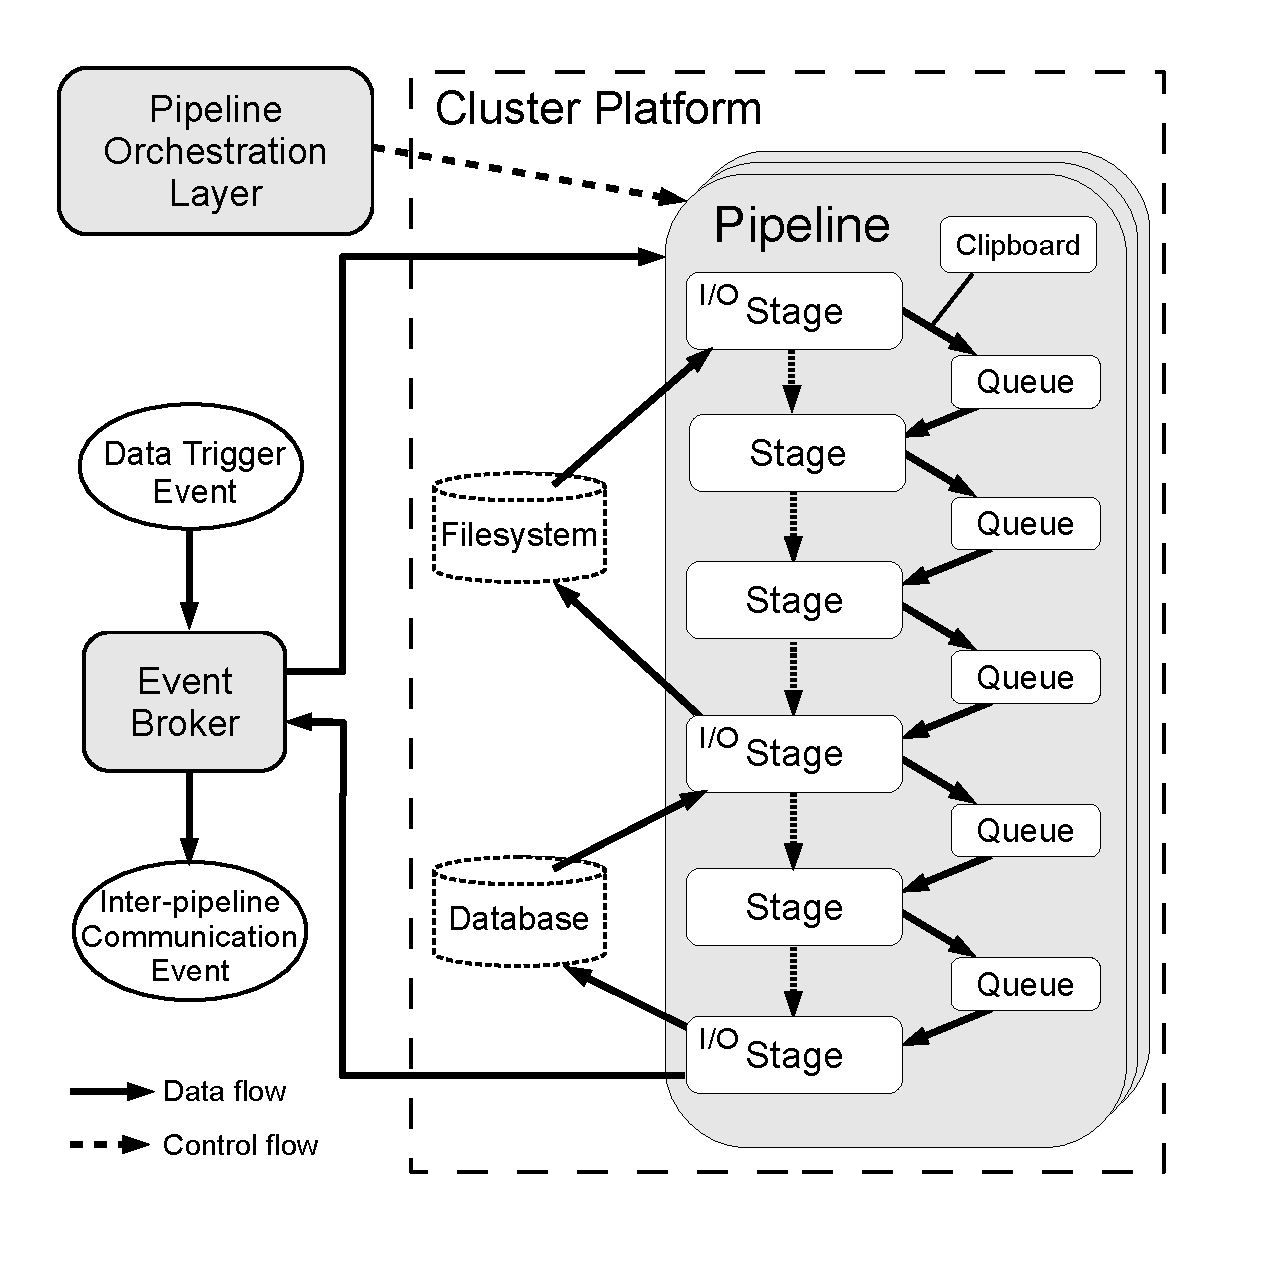
\includegraphics[height=4.0in,bb=25 45 562 583]{images/pex.pdf}
\caption{The generic pipeline framework. The pipeline orchestration
  layer launches the pipeline on a remote cluster, resulting in
  multiple parallel pipeline processes across the cluster machines.
  Processing starts when the pipeline receives a data trigger event
  via the event broker, and data and control pass through the stages.
  Some of the stages are dedicated to I/O.  The last stage can issue
  an event to trigger another pipeline to take over the processing of
  the data.
\label{fig:pex}}
\end{center}
\end{figure}

The ``science view'' of what each pipeline does in response to these
events is summarized in the subsequent sections below; however, these
actions are facilitated by the \textit{pipeline harness}, the
application container that hosts the application code which applies
the specific scientific algorithms to the data, as illustrated in
Fig. \ref{fig:pex}.  The harness runs a pipeline: it is responsible
for capturing events and making the data they contain available to the
application.  It also manages the flow of execution, executing each
stage in sequence, passing data between them, and start the sequence
over again when all the stages are done processing a chunk of data.  

Additional details of how the harness does its work can be found in
section \ref{sec:harness} and more so in the DC2 Report.  For the
discussion below, it is useful to introduce some operational concepts
that are part of the harness framework.  First, we explicitly
segregate processing into three different types of stages:  science
stages (that apply science processing algorithms to the data), I/O
stages (that read in or write out data), and miscellaneous
book-keeping stages.  This is important for our performance analysis
as we want to be able explicitly separate the effects, say, I/O from
the science algorithms.  All I/O operations, be they on files in a
filesystem or operations on a database, go through an abstract
layer referred to as \textit{persistence}.  In particular, to
\textit{persist} some data is to use the persistence layer to save a
copy of the data on disk, possibly in a database.  \textit{Loading} is to
read the data from disk and into objects in memory.  I/O is handled
through a generic stage implementation provided by the
\texttt{pex\_harness} package which can be configured via a policy to
read or write any data available via the persistence layer.  

Data objects are moved through stages attached to a \textit{clipboard}
object and transferred via \textit{queues} that connect the stages
(see fig. \ref{fig:pex}): any stage that wants to share data with
subsequent stages can ``post'' it to the clipboard and sending it to
its output queue.  In the current implementation, the clipboard is an
object in memory shared by all the stages; thus, no I/O, network
communication, or other data copying is involved in the transfer.

\subsubsection{Image Processing and Source Detection (IPSD)}

The IPSD pipeline processes images in pairs: two exposures, designated
0 and 1, are considered to have been taken consecutively with the same
field of view at essentially the same time. This pairing of exposures
allows for the detection of cosmic rays appearing in one exposure but
not the other.

The IPSD performs the following tasks, in sequence:

\begin{itemize}

\item Information is read in identifying the exposures to be processed, and 
links are created in the file system from the working directory to the input
images.

\item For image 0 of the pair, metadata in the FITS file header is read in, 
giving the exposure time, location of the field of view, and similar information, 
which is then posted to the clipboard.

\item Given this information, the calibration products associated with that
exposure are identified by lookup. Calibration products include darks,
flats, bias, and scatter exposures associated with a given camera run.

\item These calibration products are then used to perform instrument
signature removal (ISR) on the raw exposure, resulting in a calibrated image.

\item Source detection is then performed on calibrated image, giving source
information needed later for determining the WCS coordinates of the
exposure.

\item The point spread function (PSF) of the exposure is determined.

\item The second image of the pair is read in and also goes through ISR.

\item WCS of the exposures is determined.

\item The calibrated exposures are then persisted.

\item A template image representing the ideal expected exposure is
created. When processing CHFT-LS images, these templates are 
resampled from stacked images provided by the CHFT-LS survey.

\item Calibrated images 0 and 1 are subtracted from the template
image, and the difference images created are persisted.

\item These difference images are added together. Source detection
and measurement is then performed. The sources detected are
persisted in the DIASource database.

\item The association pipeline is signaled through the events broker
that the processing of the image pair is complete and that the source
data is ready for the association process.

\item SDQA data from the exposure is persisted.

\end{itemize}

\subsubsection{Night Moving Object Processing System (MOPS)}

The MOPS pipeline performs the following tasks, in sequence:

\begin{itemize}

\item Given the required field of view, MOPS predicts the positions 
of known moving objects in the field.

\item These positions are recorded into the database.

\item MOPS then signals the association pipeline, through the events
broker, that its predictions are available.

\end{itemize}

\subsubsection{Association Pipeline (AP)}

The association pipeline performs the following tasks, in sequence:

\begin{itemize}

\item The pipeline awaits signals from the event broker that
both the IPSD and MOPS pipelines have completed their computations
on a given pair of exposures.

\item New source detections from the DIASource catalog are loaded 
into memory.

\item These detections are matched against known, fixed objects.
Matches are recorded into the database.

\item The MOPS predictions for known moving objects are loaded 
into memory, and the new source detections are matched against
these predictions. Again, matches are recorded in the database.

\item New sources are then used to update the catalog of known
objects.

\end{itemize}

\subsection{Hardware Deployment}

\subsubsection{The NCSA LSST Cluster}

Most of the DC3a preliminary and production runs were performed on a dedicated 
ten-nodes Dell Server Xeon cluster hosted at NCSA. This heterogenous cluster 
consists of two Xeon 3.6 GHz single dual-core nodes, two Xeon 3.6 Ghz dual
dual-core nodes, and six Xeon 2.0 Ghz dual quad-core nodes. It uses a
gigabit ethernet interface.

This cluster was built for DC2 and the DC2 runs were performed there; for DC3, 
the cluster was upgraded from 32-bit Red Hat Enterprise Linux 4 to 64-bit
Red Hat Enterprise Linux 5. Each cluster node has 4 GB memory, with the exception
of \texttt{lsst10}, which has 16 GB. Each node has from 20 to 60 GB of local disk,
along with 15 TB of disk storage shared among nodes using the NFS shared file system.
As part of DC3a, we installed the Lustre parallel file system to increase I/O 
throughput. We were not, however, able to stabilize the Lustre installation
sufficiently to use it for production runs on the NCSA cluster, as planned.

\subsubsection{NCSA Abe}

For purposes of testing the scalability of the pipelines, additional runs were
performed on a larger cluster, Abe, hosted at NCSA. Abe consists of 1200
dual quad-core Xeon 2.33 GHz processors; for the LSST runs we used 36 of these 
nodes, for a total of 288 cores, sufficient to process an entire focal plane 
for the CHFT-LS images. Each core has 1 GB of memory, and shared access
to 100 TB of disk storage as managed using Lustre.

Abe job runs were coordinated using the Condor-G jobs management system.
The events broker and database were not moved to Abe during these runs;
they remained on the LSST cluster.
